\documentclass[../thesis.tex]{subfiles}

\begin{document}

Steady progress in any modern scientific endeavor requires a strong, dynamic relationship between experimental data to paint an accurate picture of some natural phenomena and theoretical models to interpret those phenomena with respect to the growing network of other scientific models. Conversely, the predictive capability of theoretical models can highlight blurry or unfinished areas of that picture which can be clarified or completed by new or improved experimental techniques. In the pursuit to understand and describe the atomic nucleus and the corresponding implications from quarks to neutron stars, this push-and-pull coordination between theory and experiment makes progress in modern nuclear physics robust and persistent.

An integral component of modern nuclear physics is describing the structure and emergent properties of self-bound systems of protons and neutrons. The systems in questions can be stable nuclei, rare isotopes far from stability, and even infinite nuclear matter which can be used to model neutron stars. Relevant properties to nuclear structure include ground-state energies--for determining nuclear masses, excited-state energies--for identification in gamma or neutron spectroscopy, and transition or decay amplitudes--for calculating the respective rates for those processes. This wide array of emergent properties inserts both nuclear structure theory and experiment into a prominent role within every other subfield of modern nuclear physics, from lattice quantum chromodynamics (QCD) to nuclear astrophysics, and beyond, to questions about fundamental symmetries and dark matter.  However, two inextricable characteristics of a comprehensive model of nuclear structure--the increasingly large size of many-body nuclear systems and the complexity and strength of the nucleon-nucleon interactions--have been imposing hurdles for theorists to overcome.


\section{A Brief History of Nuclear Structure Theory}

The project to solve the correlation problem in many-fermion systems began with the work of Brueckner, Bethe, and Goldstone \cite{BRUECKNER19551344,BETHE19561353,GOLDSTONE1957267} with the reformulation of the nuclear interaction by accounting for two-body correlations from the nuclear medium.  This work continued with the work of Coester and Kummel \cite{COESTER1958421,COESTER1960477,KUMMEL19781} with a further resummation of nuclear correlations in the form of an exponential ansatz into what would become coupled-cluster (CC) theory.  However, there were two major obstacles that hindered the progress in this area for decades.  First, while these methods were systematically improvable by including progressively higher-level correlations, the highly-nonperturbatuve nature of the nuclear force required computationally infeasible summations.  Second, there wasn't a reliable and consistent theory to model nucleon-nucleon interactions.

\begin{figure}[h]
  \centering
  \begin{subfigure}{0.65\textwidth}
    \centering
    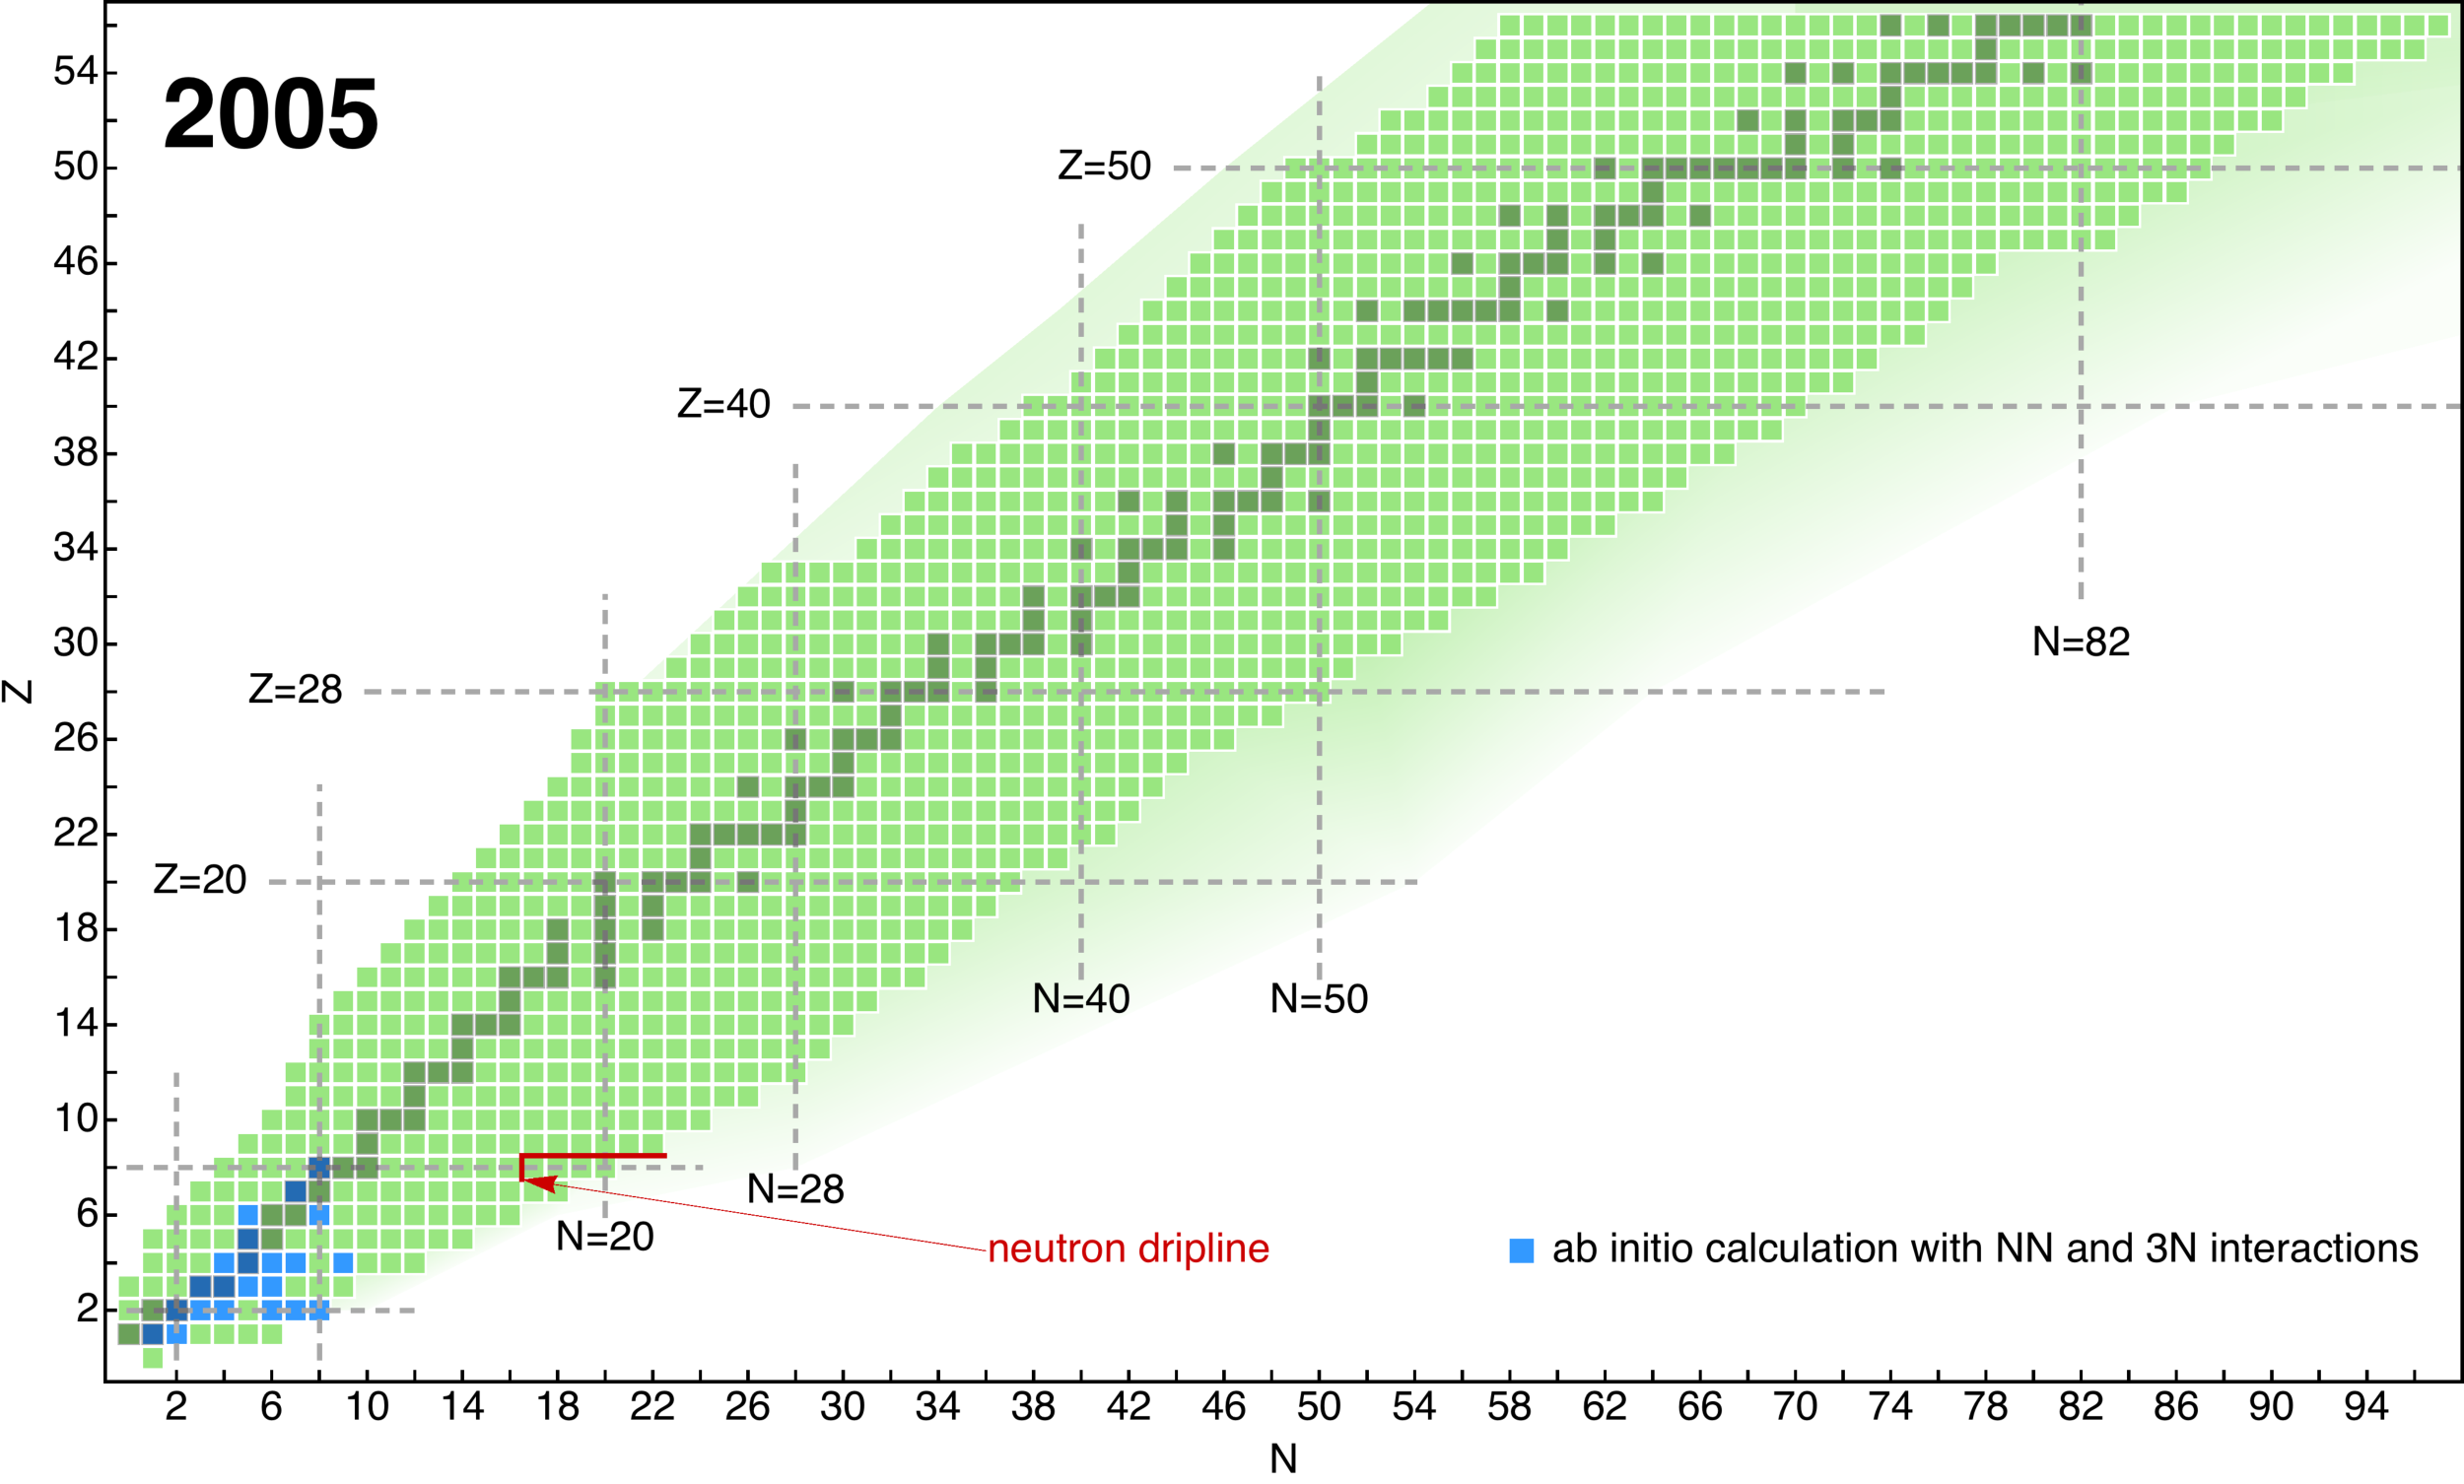
\includegraphics[width=\textwidth]{introduction/ab-initio_nuclear_chart_2005.pdf}
  \end{subfigure}
  
  \begin{subfigure}{0.65\textwidth}
    \centering
    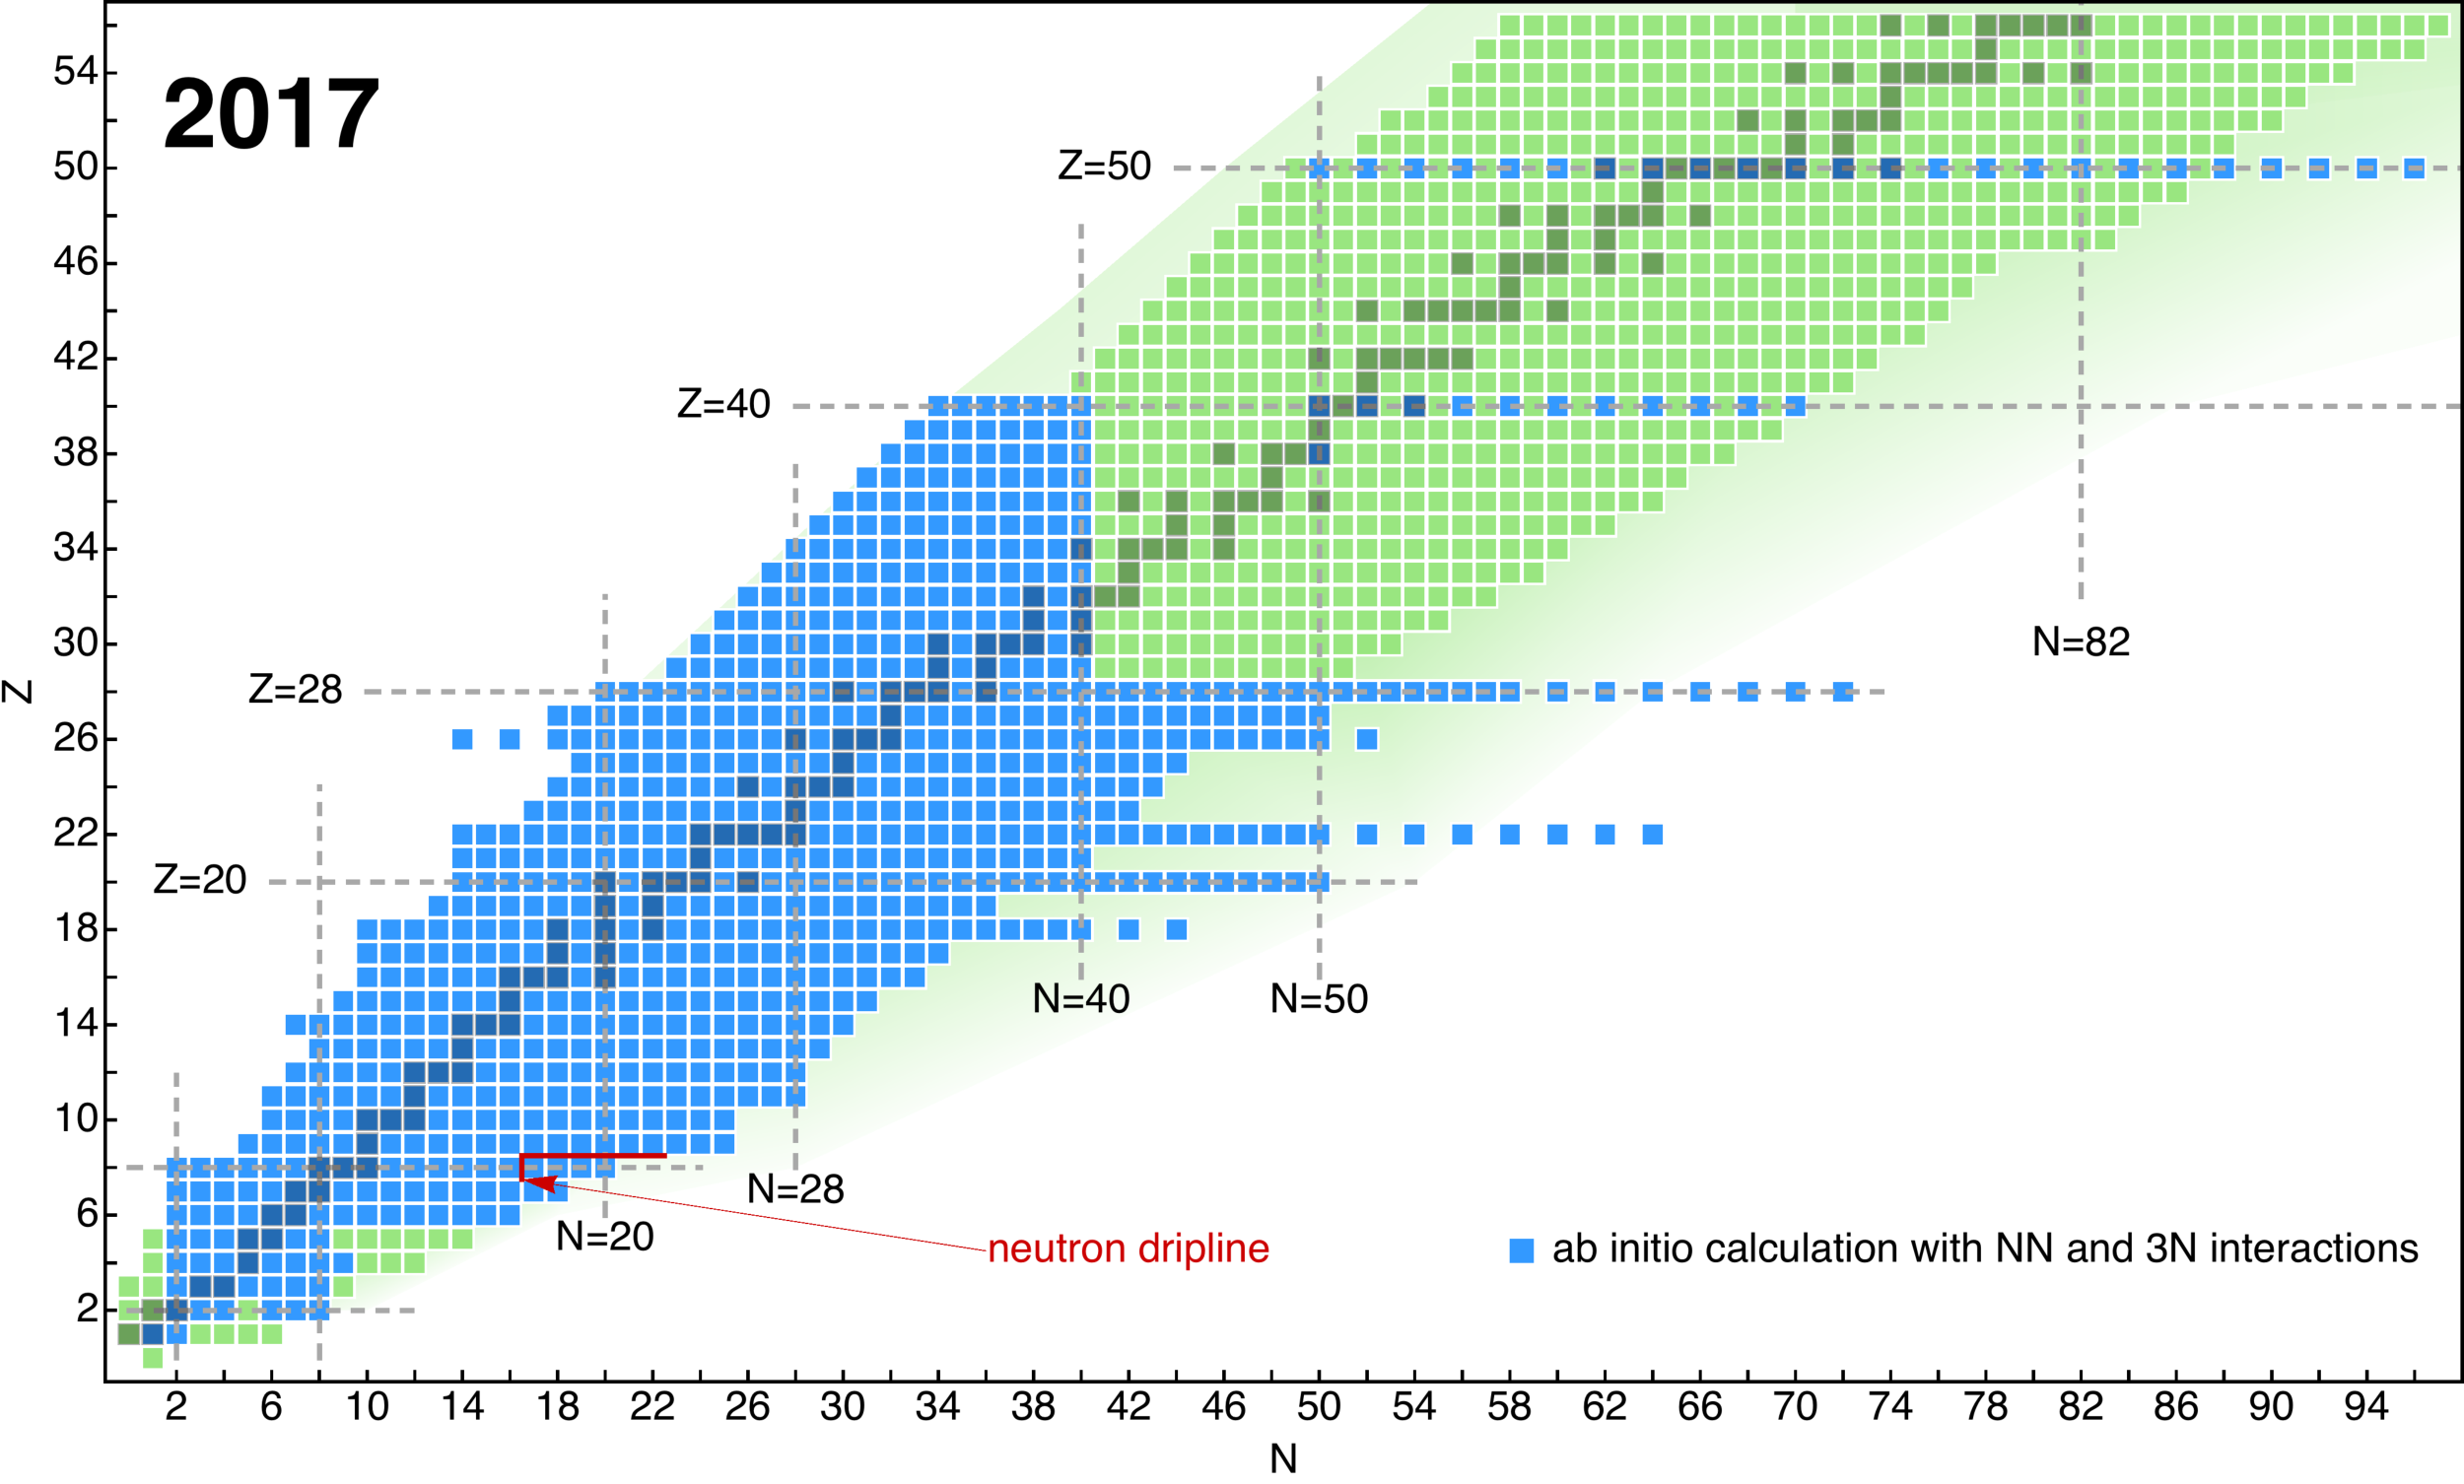
\includegraphics[width=\textwidth]{introduction/ab-initio_nuclear_chart_2017.pdf}
  \end{subfigure}
  \caption{Nuclear chart of nuclei with ground-state energies which have been calculated with ab-initio methods and NN+3N interactions.  Figure taken from \cite{HERGERTPRIVATE}.}
  \label{fig:AbInitioChart}
\end{figure}

However, the well-known and highly-perturbative Coulomb force, which underlies the many-electron systems in atoms and molecules, made consistent advances in ab-initio quantum chemistry possible since the 1950s.  Along with the quasi-exact method of configuration interaction (CI) \cite{SLATER19291293,CONDON19301121,BACHER1933264,UFFORD1933732} which physicists hav utilized since the formulation of quantum mechanics, chemists successfully employed approximate methods like many-body perturbation theory (MBPT) \cite{HUBBARD1957539,HUGENHOLTZ1957481,SCHAEFER1984,SHAVITT2009} and coupled-cluster theory \cite{CIZEK19664256,CIZEK1971359,CIZEK1980251,PIECUCH2002527,SHAVITT2009}.

Fortunately, within the past decade, two breakthroughs have allowed ab-initio nuclear structure to resurface and thrive the way that quantum chemistry had done.  The first was the invention of chiral effective field theory (EFT) \cite{EPELBAUM20091773,MACHLEIDT20111} which gave theorists the ability to construct nucleon-nucleon interactions consistent with the underlying QCD of the strong nuclear force.  The second was the application of renormalization group (RG) methods to the nuclear force \cite{BOGNER201094,ROTH2011072501}.  This procedure can ``soften'' the NN interaction, to decouple the high- and low-momentum components of the nuclear force and generate less-correlated systems that can be calculated at a reasonable computational cost.  These major changes to nuclear structure theory made it possible to merge the field with the progress of quantum chemistry and open a new area for additional developments in ab-initio descriptions of many-fermion systems.

no-core shell model NCSM \cite{NAVRATIL2000054311,NAVRATIL2009083101,BARRETT2013131}
quantum Monte Carlo QMC \cite{PUDLINER19971720,PIEPER200153,CARLSON20151067}

modern CC \cite{WLOCH2005212501,WLOCH2005S1291,JANSEN2014142502,JANSEN2016011301,HAGEN2015186,KOWALSKI2004132501,GOUR2006024310,BINDER2013054319}
modern IMSRG \cite{TSUKIYAMA2011222502,TSUKIYAMA2012061304,HERGERT2013242501,BOGNER2014142501,HERGERT2014041302,HERGERT2017023002,STROBERG2016051301,STROBERG2017032502}
self-consistent Green's function SCGF \cite{SOMA2013011303,SOMA2014024323,SOMA2014061301}

\begin{figure}[h]
  \centering
  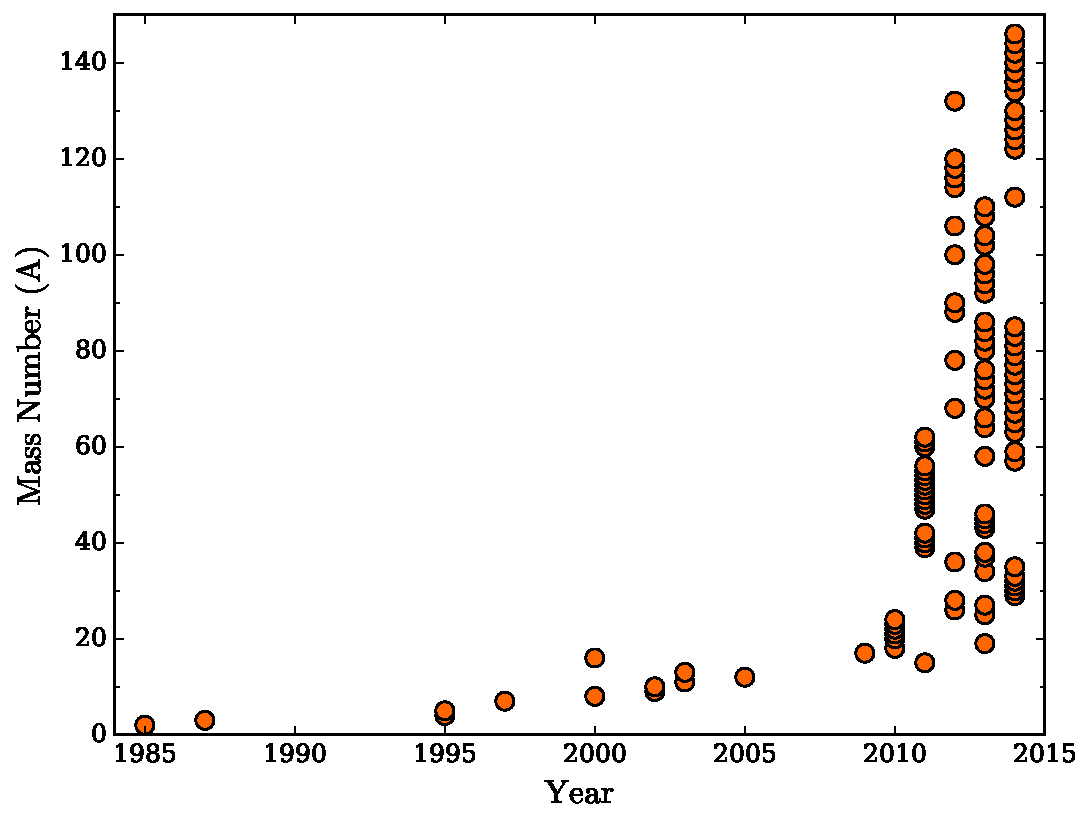
\includegraphics[width=0.75\textwidth]{introduction/ab-initio_progress.pdf}
  \caption{Progress of ab-initio nuclear structure from calculations of ground-state energies with NN+3N interactions.  Early progress was approximately linear as the problem size scaled with Moore's law while more recent progress has taken advantage of new algorithms which have outpaced Moore's law.  Data taken from \cite{HERGERTPRIVATE}.}
  \label{fig:AbInitioProgress}
\end{figure}


\section{Electroweak Theory and Nuclear Structure}

Nuclear structure is implicated in performing and analyzing experiments to probe fundamental symmetries and physics beyond the Standard Model. One example is determining the $\mathrm{V_{ud}}$ component of the Cabbibo-Kobayashi-Maskawa (CKM) matrix, which relates quark eigenstates of the weak interaction to their mass eigenstates \cite{CABBIBO1963531,KOBAYASHI1973652}. This matrix element can be determined from by measuring the half-lives of superallowed Fermi beta decays \cite{TOWNER2003197} and applying a nucleus-dependent structure correction \cite{TOWNER2008025501,TOWNER199413,TOWNER1992478,BARKER1992501,JAUS1990166}. The value of $\left|\mathrm{V_{ud}}\right|$ is used to test the unitarity of the CKM matrix and the conserved-vector current hypothesis, which relates the $f$t-values of superallowed Fermi beta decays of different nuclei, both predicted by the standard model \cite{HARDY2005055501}.

Another example of physics beyond the standard model is the neutrinoless double-beta decay ($0\nu\beta\beta$) \cite{SUHONEN1998123,AVIGNONE2008481}. The extremely-rare, two-neutrino double-beta decay ($2\nu\beta\beta$) has been observed in many experiments \cite{ELLIOTT19872020,MILEY19903092}, which has motivated the search for its neutrinoless counterpart, in which two Majorana neutrinos--being their own antiparticles--annihilate one another, which is not possible in the standard electro-weak theory. The long half-lives of these theoretical decays depend on a phase-space factor, which is highly dependent on the decay $Q$-value, and a nuclear matrix element. The $Q$-value can be determined from high-precision mass measurements of the relevant nuclei \cite{LINCOLN2013012501,GULYUZ2015055501,REDSHAW2012041306,BUSTABAD2013022501}, while the nuclear matrix element, which contributes the largest source of uncertainty, must be calculated with a sufficient many-body theory. 

The weak interaction and nuclear structure can also be exploited for supernova neutrino detection and spectroscopy. While these original detectors were based on electron-neutrino scattering \cite{HIRATA19871490,BIONTA19871494}, more recent experiments utilize correlated nucleon effects of large nuclei to enhance the scattering cross section and therefore the ability to resolve energies and distinguish neutrino flavors \cite{HARGROVE1996183,CLINE1994720,EWAN1992373,LANGANKE19962629}. Supernova models predict distinct distributions for different neutrino flavors based on the temperatures at which they are emitted \cite{KOLBE20032569,BENHAR2005053005}. With nuclear structure calculations that include sufficient nuclear correlations, these high-resolution detectors can be used to verify specific models.


\section{Ab-Initio Descriptions of Beta Decay}

The ab-initio calculations needed in order to contribute to new endevours on the cutting edge of physics research.


\section{Thesis Structure}

The main goal of this work is to explore the ab-initio description of nuclear beta decay within the coupled-cluster theory framework of EOM-CCSD using renormalized chiral NN and 3N interactions.  The organization of the thesis builds from a general description of the many-body problem of quantum mechanics in chapter \ref{chapter:manybody}. Then, in chapter \ref{chapter:cc}, this many-body framework is applied within the coupled-cluster theory an applied to various systems including atomic nuclei. In chapter \ref{chapter:eom}, coupled-cluster theory is extended to the equations-of-motion method to describe open-shell systems.  Chapter \ref{chapter:effectiveoperators} outlines the procedure to express observables as effective coupled-cluster operators and how to calculate those observables in the equations-of-motion framework.  Then, in chapter \ref{chapter:betadecay}, the ability to calculate effective operators is applied to Fermi- and Gamow-Teller- beta-decay operators and relevant quantities are determined for various nuclei.  Lastly, conclusions and future perspectives are given in chapter \ref{chapter:conclusions} while technical details concerning the formalism and implementation are given in the appendix \ref{chapter:appendix}.

\end{document}
